\documentclass[pdflatex,11pt]{aghdpl}
% \documentclass{aghdpl}               % przy kompilacji programem latex
% \documentclass[pdflatex,en]{aghdpl}  % praca w języku angielskim
\usepackage[polish]{babel}
\usepackage[utf8]{inputenc}

% dodatkowe pakiety
\usepackage{enumerate}
\usepackage{listings}
\lstloadlanguages{TeX}

\lstset{
  literate={ą}{{\k{a}}}1
           {ć}{{\'c}}1
           {ę}{{\k{e}}}1
           {ó}{{\'o}}1
           {ń}{{\'n}}1
           {ł}{{\l{}}}1
           {ś}{{\'s}}1
           {ź}{{\'z}}1
           {ż}{{\.z}}1
           {Ą}{{\k{A}}}1
           {Ć}{{\'C}}1
           {Ę}{{\k{E}}}1
           {Ó}{{\'O}}1
           {Ń}{{\'N}}1
           {Ł}{{\L{}}}1
           {Ś}{{\'S}}1
           {Ź}{{\'Z}}1
           {Ż}{{\.Z}}1
}

%---------------------------------------------------------------------------

\author{Ksawery Głaz}

\titlePL{Analiza wpływu składowych systemu rozszerzonej rzeczywistości na jakość uzyskiwanego obrazu.}
% \titleEN{}

% \shorttitlePL{Przygotowanie pracy dyplomowej w~systemie \LaTeX} % skrócona wersja tytułu jeśli jest bardzo długi
% \shorttitleEN{Thesis in \LaTeX}

\thesistypePL{Praca magisterska}
% \thesistypeEN{Master of Science Thesis}

\supervisorPL{prof. dr hab. inż. Krzysztof Boryczko}
% \supervisorEN{Marcin Szpyrka Ph.D}

\date{2016}

\departmentPL{Katedra Informatyki}
% \departmentEN{Department of Automatics}

\facultyPL{Wydział Informatyki, Elektroniki i Telekomunikacji}
% \facultyEN{Faculty of Electrical Engineering, Automatics, Computer Science and Electronics}

% \acknowledgements{Serdecznie dziękuję \dots tu ciąg dalszych podziękowań np. dla promotora, żony, sąsiada itp.}


\setlength{\cftsecnumwidth}{10mm}

%---------------------------------------------------------------------------

\begin{document}

\titlepages

\tableofcontents
\clearpage

\chapter{Wprowadzenie}
\label{cha:wprowadzenie}

\par
Modelowanie w ostatnich latach stało się istotnym zagadnieniem w wielu dziedzinach naukowych. Podstawowym celem modelowania stało się uproszczenie rzeczywistości umożliwiające poddanie jej procesowi badawczemu. Takie podejście umożliwia między innymi analizę zjawiska będącego przedmiotem badań w zmienionej skali czasowo-przestrzennej, adekwatną zmianę skali obiektu badań, analizę procesów zachodzących w skalach czasowych rzędu nano- lub mikrosekund czyli trudnych do uchwycenia w warunkach laboratoryjnych. Modelowanie umożliwia również badanie wybranego, jednego aspektu zagadnienia będącego przedmiotem analizy.
\par
Odrębnym zagadnieniem w technikach modelowania jest modelowanie obiektów i scen trójwymiarowych. Dotyczy ono tworzenia obiektów i scen wykorzystujących głównie obiekty dostępne w bibliotekach różnych programów i zasadniczo ogranicza się do scen statycznych. Znacznie bardziej ciekawym rozwiązaniem jest propozycja połączenia scen pochodzących ze świata rzeczywistego z obiektami lub scenami generowanymi komputerowo. Klasyczne w tym zakresie rozwiązania bazują na połączeniu obrazu świata rzeczywistego dostarczanego przez kamerę z generowaną w czasie rzeczywistym grafiką 3D. Należy zwrócić uwagę, iż obraz świata rzeczywistego może być dostarczany przez sygnały o różnych częstotliwościach podstawowych. Spotyka się również rozwiązania, w których wykorzystywana jest fuzja sygnałów z kamer pracujących w zakresie fal widzialnych dla człowieka oraz fal radiowych. Powstały w ten sposób obraz określa się rozszerzoną rzeczywistością (ang. Augmented Reality).
\par
W literaturze można spotkać wiele definicji rozszerzonej rzeczywistości. Najistotniejsze wydają się być jednak wymagania stawiane tego typu systemom. Wśród najważniejszych należy wymienić przede wszystkim łączenie świata rzeczywistego z wirtualnym, konieczność pracy w czasie rzeczywistym oraz umożliwianie ruchów każdego elementu w trzech wymiarach.
\par
Pozornie prosty postulat dotyczący łączenia scen świata rzeczywistego z generowanymi scenami wirtualnymi kryje w sobie konieczność rozwiązania szeregu problemów naukowych oraz technologicznych. Efektywność zaproponowanych w tym zakresie metod przekłada się bezpośrednio na jakość uzyskanej sceny (modelowania). Dodatkowe ograniczenie wymuszające konieczność generowania wynikowej sceny w czasie rzeczywistym wymusza użycie właściwych dla danego zastosowania algorytmów dedykowanych dla danej architektury sprzętowej oraz ich specyficzną implementację.

%---------------------------------------------------------------------------

\section{Cele pracy}
\label{sec:celePracy}

Celem głównym niniejszej pracy jest stworzenie systemu do tworzenia aplikacji z zakresu rozszerzonej rzeczywistości. Szczególny nacisk zostanie położony na jakość uzyskiwanych scen, co jest zdeterminowane głównie precyzją łączenia obrazu rzeczywistego i scen wirtualnych. Dla tak zaproponowanego celu ogólnego zrealizowano kilka celów szczegółowych. Należą do nich:
\begin{itemize}
	\item Analiza dostępnych algorytmów łączenia obrazu rzeczywistego i scen generowanych.
	\item Analiza metod oceny jakości sceny rozszerzonej rzeczywistości oraz propozycja własnych kryteriów w tym zakresie.
	\item Propozycja własnych algorytmów dla metod rozszerzonej rzeczywistości uwzględniających określone kryteria jakości.
	\item Ocenę jakości zaproponowanych algorytmów.
	\item Sformułowanie ogólnych zasad tworzenia aplikacji dla przedmiotowego zakresu.
\end{itemize}

%---------------------------------------------------------------------------

\section{Zawartość pracy}
\label{sec:zawartoscPracy}

Niniejsza praca zawiera opis realizacji merytorycznie spójnych etapów koniecznych dla stawianego celu ogólnego. W rozdziale pierwszym ....



\chapter{Przegląd istniejących rozwiązań w zakresie rozszerzonej rzeczywistości}
\label{cha:przegladIstniejacychRozwiazanWZakresieRozszerzonejRzeczywistosci}

W tym rozdziale zostało omówione kilka bibliotek implementujących narzędzia wykorzystywane w rozszerzonej rzeczywistości. W internecie można znaleźć dużo w tym także darmowych i open source bibliotek, które możemy wykorzystać do różnych programów na przykład gier, które wykorzystują rozszerzoną rzeczywistość.

%---------------------------------------------------------------------------

\section{Ogólne założenia systemów rozszerzonej rzeczywistości}
\label{sec:ogolneZalozeniaSystemowRozszerzonejRzeczywistosci}

Na początku warto wspomnieć o kilku ogólnych założeniach, które charakteryzują systemy rozszerzonej rzeczywistości. Poniżej w kilku punktach zostało opisane kilka cech takich systemów:
\begin{itemize}
	\item Obraz wirtualny bądź jego elementy nakładane są na obraz rzeczywisty uzyskany z kamery. Najczęściej punktem odniesienia są różnego rodzaju markery, jednakże mogą to być także różne charakterystyczne przedmioty otoczenia z pozyskanego obrazu rzeczywistego.
	\item Jednym z najtrudniejszych elementów w rozwijaniu aplikacji wykorzystujących rozszerzoną rzeczywistość jest dokładne obliczanie punktu widzenia użytkownika w czasie rzeczywistym, dzięki czemu wirtualne obrazy są dokładnie dostosowane do rzeczywistych obiektów.
	\item Obraz rzeczywisty ma zazwyczaj bardziej skomplikowane wymagania kalibracji kamery i rejestracji obrazu.
	\item Każdy z takich systemów wymaga kalibracji kamery, aby przy rozpoznawaniu obrazów można łatwo było określić położenie i orientację markerów, oraz odpowiednio wyświetlać przypisane im obiekty wirtualne. Niektóre z tych systemów posiadają własną implementację umożliwiającą taką kalibrację. 
	\item Biblioteki opierające się na markerach, rozpoznają je najczęściej poprzez przetworzenie obrazu rzeczywistego na obraz binarny (czarno-biały) i znajdują w ten sposób czarną ramkę ograniczającą dany marker, a następnie zajmują się ich identyfikacją.
\end{itemize}

%---------------------------------------------------------------------------

\section{ARToolkit}
\label{sec:artoolkit}

Jest to jedna z najbardziej popularnych bibliotek open source wykorzystywanych w rozszerzonej rzeczywistości. Posiada także wiele rozszerzeń takich jak FLARToolkit i wiele podobnych. Kod źródłowy dla tego projektu jest zamieszczony na GitHub \cite{ARToolkit}, skompilowane SDK dla wszystkich platform (Mac OS X, PC, Linux, Android, iOS) wraz z wtyczką dla ARToolKit Unity3D, dostępne są na stronie głównej projektu \cite{ARToolkit}. Zaletami tej biblioteki są:
\begin{itemize}
	\item Solidne śledzenie markerów.
	\item Dobre wsparcie kalibracji kamery.
	\item Wieloplatformowe oraz posiada wpsarcie dla wielu języków programowania.
	\item Zoptymailizowane dla urządzeń mobilnych.
	\item Wsparcie dla unity3D oraz OpenSceneGraph.
\end{itemize}

ARToolKit wykorzystuje techniki wizualizacji komputerowej by obliczyć pozycję kamery i orientację względem kwadratowych kształtów lub płaskich powierzchni teksturowanych, pozwalając programiście nakładanie wirtualnych przedmiotów. ARToolKit obsługuje obecnie klasyczny kwadratowy znacznik, kod kreskowy 2D, wiele innych rodzajów markerów. Ponadto ARToolKit obsługuje dowolną kombinację powyższych razem. Szybkie, precyzyjne śledzenie dostarczone przez ARToolKit umożliwiło szybki rozwój tysiącu nowych i ciekawych aplikacji rozszerzonej rzeczywistości. ARToolkit obsługuje zarówno pliki wideo jaki obraz rzeczywisty bezpośrednio z kamerki.

Biblioteka opiera się na kwadratowych markerach składających się z białego tła oraz posiadających szeroką ciemną (zazwyczaj czarną) otoczkę wytyczającą granice markera. Konstrukcja ta czyni marker wyjątkowym, łatwym do rozpoznania. Są one rozpoznawane, wykrywane, a następnie używane do obliczania położenia w przestrzeni 3D. ARToolkit działa następująco:
\begin{itemize}
	\item Aparat rejestruje wideo w polu widzenia kamery i wysyła je do komputera.
	\item Oprogramowanie na komputerze przeszukuje każdą klatkę wideo dla dowolnych kształtów kwadratowych (markery kwadratowe).
	\item Jeśli kwadratowy marker zostanie znaleziony i treść obrazu osadzona przez wzór, jest dopasowana i zidentyfikowana to oprogramowanie wykorzystuje matematykę do obliczenia, w stosunku do aparatu, zarówno pozycję czarnego kwadratu jak i orientację wzoru.
	\item Gdy pozycja i orientacja kamery są znane, model grafiki komputerowej jest rysowany za pomocą położenia obliczonej pozycji i orientacji dopasowania.
	\item Model ten jest rysowany w planie przechwyconego wideo i są śledzone ruchy wideo w tle, a następnie model jest dołączany do tła.
	\item Wynikiem końcowym jest pokazany na wyświetlaczu obiekt w tle obrazu z kamery, więc widz widzi renderowany graficzny model nad strumieniem wideo świata rzeczywistego.
\end{itemize}

\begin{figure}[ht!]
\centering
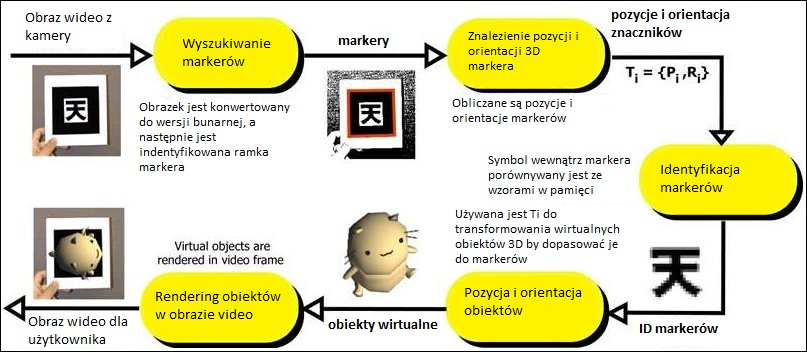
\includegraphics[width=150mm]{diagram.jpg}
\caption{Działanie ARToolkit krok po kroku \label{artoolkitSteps}}
\end{figure}

Rysunek \ref{artoolkitSteps} podsumowuje powyższe kroki.
\bigskip

ARToolkit posiada jednak pewne ograniczenia. Obiekt wyświetlany jest tylko wtedy gdy marker jest w polu widzenia kamery. Jeżeli choć część markera zostanie czymś przysłonięta to wirtualny obiekt znika. Natomiast jeżeli granice markera będą poza polem widzenia kamery to obiekt zostanie obcięty. Istnieje również problem w zakresie śledzenia optycznego, ponieważ kiedy markery są przeniesione dalej od kamery to znaczniki zajmują mniej pikseli widzenia kamery i wynikiem jest posiadanie niewystarczającej ilości szczegółów by wyśledzić i zidentyfikować marker. Im większy fizycznie osadzony wzór markera tym dalej wzór markera można wykryć, a więc większa umiejętność wykrywania markera. Wreszcie, wyniki śledzenia są również zależne od warunków oświetleniowych. Zbyt mocne oświetlenie może tworzyć odbicia i odblaski (plamy) na paierowych markerach i tak sprawiają, że trudniej znaleźć kwadratowy marker. Cienie mogą być rzucone w poprzek papieru, rozbijając białe obszary na obrazie z kamery.

% %---------------------------------------------------------------------------

\section{ArUco}
\label{sec:aruco}

Podobnie jak ARToolkit biblioteka ArUco opiera sie na kwadratowych znaczniakach ograniczonych czarną ramką. Jest to prosta biblioteka napisana w C++ umożliwiająca detekcję markerów za pomocą niewielkiej ilości kodu. Biblioteka także nie jest bardzo wymagająca, gdyż potrzeba doinstalować tylko bibliotekę OpenCV, na której się ona opiera. Powstały także implementacje w językach Java (dokumentacja tylko w języku hiszpańskim na stronie twórców projektu) i Python, tak więc korzystanie z biblioteki jest możliwe na każdej platformie, na której da się zainstalować i skonfigurować bibliotekę OpenCV. Niestety nie ma możliwości aby wykorzystać ArUco do programowania aplikacji mobilnych. Zdecydowaną zaletą tego projektu jest uproszczona budowa markerów, które kodowane są binarnie za pomocą białych i czarnych pól kwadratowych wewnątrz ramki. Dodatkowo prosta instalacja oraz przykładowe programy podane na stronie producentów biblioteki \cite{ArUco} powodują, że zapoznanie się oraz jej użytkowanie jest dużo łatwiejsze i przyjemniejsze.
\bigskip

\begin{figure}[ht!]
\centering
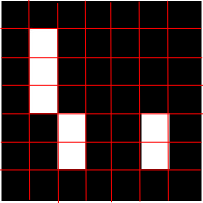
\includegraphics[width=50mm]{aruco-marker.png}
\caption{Przykładowy marker rozpoznawany przez ArUco. \label{arucoMarker}}
\end{figure}

Jak widać na rysunku \ref{arucoMarker} kwadratowy marker możemy podzielić siatką na mniejsze równych rozmiarów kwadraty (dokładnie 7x7) jednakże te brzegowe są poświęcone na ramkę markera, tak więc mamy 5x5 pól do binarnego kodowania znacznika (gdzie pole czarne oznacza 0, a pole białe 1) co powinno ułatwić, a nawet przyspieszyć jego detekcję. Każdy marker zawiera kod, który składa się z 5 słów, po pięć bitów każde. Pojedyńcze słowo ma przeznaczone 2 bity na informację oraz 3 pozostałe do detekcji błędów. Dzięki temu możemy uzyskać 2\textsuperscript{10} różnych id.
\bigskip

Detekcja markerów w ArUco przebiega następująco:
\begin{figure}[ht!]
\centering
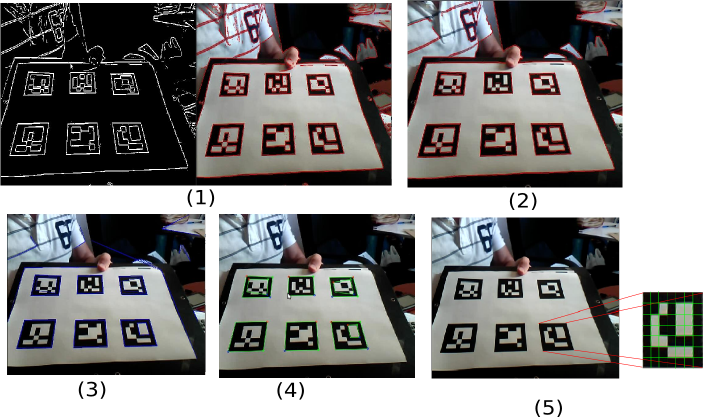
\includegraphics[width=100mm]{aruco-detection.png}
\caption{Detekcja markerów w ArUco. \label{arucoDetection}}
\end{figure}

\begin{itemize}
	\item Zamieniamy uzyskany z kamery obraz na obraz binarny.
	\item Dla uzyskanego czarno-białego obrazu stosujemy Adaptive Thresholding by wykryć wszystkie krawędzie (Zdjęcie (1) na obrazku \ref{arucoDetection}).
	\item Wykrywamy kontury. Po tym kroku mamy wykryte nie tylko kontury markerów, ale także różne inne nie potrzebne nam kontury, dlatego musimy je przefiltrować:
	\begin{itemize}
		\item Usuwamy krawędzie z małą liczbą punktów (Zdjęcie (2) na obrazku \ref{arucoDetection}).
		\item Aproksymujemy łamane konturów i zachowujemy tylko te, które posiadają dokładnie 4 wypukłe rogi (Zdjęcie (3) na obrazku \ref{arucoDetection}).
	\end{itemize}

	\item Sortujemy uzyskane rogi w kierunku przeciwnym do wskazówek zegara.
	\item Usuwamy z prostokąty znajdujące się zbyt blisko siebie ponieważ Adaptive Thresholding wykrywa też prostokąty wewnętrzne w markerach (Zdjęcie (4) na obrazku \ref{arucoDetection}).
	\item Identyfikujemy markery:
	\begin{itemize}
		\item Usuwamy perspektywę projekcji (kamera może nie być ustawiona prostopadle do markera) aby uzyskać widok prostopadły markera (Zdjęcie (5) na obrazku \ref{arucoDetection}).
		\item Dzielimy marker za pomocą algorytmu Otsu na macierz czarnych i białych kwadratowych pól.
		\item Identyfikacja kodu wewnątrz markera z pominięciem ramki.
	\end{itemize}

	\item Dla prawidłowych markerów analizujemy rogi używając interpolacji subpikseli.
	\item Na końcu obliczamy współrzędne markerów w obrazie kamery poprzez jej parametry uzyskane w kalibracji.
\end{itemize}

Kolejną zaletą ArUco w przeciwieństwie do ARToolkit jest fakt, że jeżeli w trakcie nagrywania obrazu zostanie przysłonięta część markera to obiekt nie znika całkowicie tylko jest przysłaniany, co obrazuje chociażby przykładowa aplikacja do gry w szachy wykorzystująca ArUco \cite{AugmentedRealityChess} jak i kilka innych przykładów podanych na stronie twórców \cite{ArUco}. Jedną z drobnych niedogodności mogą być warunki oświetleniowe. Jeżeli marker zostanie oświetlony mocnym stumieniem światła to na obrazie pojawi się wielka biała plama w tym miejscu.

% %---------------------------------------------------------------------------

\section{Vuforia}
\label{sec:vuforia}

Ostatnią wybraną biblioteką jest Vuforia. Jest to biblioteka, która umożliwa rozpoznawać obrazki i obiekty oraz rekonstuować elementy świata rzeczywistego. Na stronie projektu \cite{Vuforia} możemy pobrać aplikację, a także przeczytać dość obszernie opis produktu. Mamy do wyboru kilka wersji, najbardziej podstawowa Starter jest darmowa, jednak za pozostałe jej wersje Classic i Cloud trzeba zapłacić dość nie małe ceny. Niestety mimo iż jest biblioteką częściowo darmową to nie pozwala na modyfikacje jej implementacji gdyż nie jest open-source. Posiada jednak bardzo rozbudowane formy detekcji w porównaniu z dwoma poprzednimi bibliotekami. Może rozpoznawać takie elementy jak:
\begin{itemize}
	\item Płaskie wydrukowane obrazki, które także mogą pełnić rolę markerów.
	\item Wiele obrazków na raz np. pudełko składające się z obrazków.
	\item Obiekty o kształtach walcowatych np. kubki, piszki itp.
	\item Markery w ramkach - udostępnia 512 numerycznie zakodowanych markerów.
	\item Teksty - rozpoznaje około 100 tysięcy angielskich słów ze słownika.
	\item Róznego rodzaju obiekty 3D.
\end{itemize}

Platforma składa się z 3 głównych elementów:
\begin{itemize}
	\item The Vuforia Engine - jest to biblioteka od strony klienta statycznie połączona z tworzoną aplikacją za pomocą Vuforii.
	\item Tools - środowisko zapewnia narzędzia do tworzenia celów do wykrywania (markerów, obrazków), zarządzania bazą danych je zawierającą czy też do zabezpieczania licencji aplikacji.
	\item Cloud Recognition Service - serwis wykorzystywany gdy aplikacja potrzebuje przetwarzać duże zbiory obrazów lub baza danych jest często uaktualniana.
\end{itemize}

Vuforia jest dość mocno rozbudowaną biblioteką dającą sporą ilość możliwości do wykorzystania w aplikacjach opartych na systemach rozszerzonej rzeczywistości. Jeżeli dana aplikacja nie będzie korzystana do celów komercyjnych możemy korzystać z tej biblioteki za darmo (będzie ona dołączać znak wodny), jeżeli jednak chcemy użyć jej do celów komercyjnych to jest ona dość kosztowna zwłaszcza jeżeli chcemy ją wykorzystać do aplikacji które są często aktualizowane. Na stronie projektu \cite{Vuforia} możemy także znaleźć opis jak zainstalować aplikację oraz przykładowe aplikacje korzystające z tej biblioteki, które dobrze prezentują jej możliwości.

% %---------------------------------------------------------------------------

\section{Podsumowanie}
\label{sec:podsumowanie}

Obecnie rozszerzona rzeczywistość rozwija się dość szybko by spełniać oczekiwania społeczeństwa, w którym rozwój technologiczny postępuje coraz szybciej. Przedstawione powyżej biblioteki stanowią tylko niewielką część wszystkich systemów, które rozwijają zagadnienie rozszerzonej rzeczywistości. Każda z nich daje różne możliwości rozwiązań co można zobaczyć w tabeli porównującej je \ref{tab:tabelaPodsumowania}.

\begin{table}[h!]
	\begin{center}
		\begin{tabular}{| p{35mm} | p{35mm} | p{35mm} | p{35mm} |}
			\hline
			\textbf{Cecha} & \textbf{ARToolkit} & \textbf{ArUco} & \textbf{Vuforia} \\ \hline
			Otwarty kod & \multicolumn{2}{c|}{Tak} & Nie \\ \hline
			Płatna & \multicolumn{2}{c|}{Nie} & Tylko w celach komercyjnych \\ \hline
			Rozpoznawanie obrazu & \multicolumn{2}{c|}{Tylko markery} &  Markery i obiekty z obrazu \\ \hline
			Rodzaje markerów & Ograniczone grubą czarną ramką z dowolną zawartością wewnątrz & Ograniczone czarną ramką z pięcioma zakodowanymi binarnie słowami w postaci czarnych i białych kwadratów & Rozpoznaje markery ze swojej bazy markerów, płaskie obrazy oraz obiekty 3D także mogą pełnić rolę markerów \\ \hline
			Wieloplatformowe & \multicolumn{3}{c|}{Tak} \\ \hline
			Aplikacje mobilne & Tak & Nie & Tak \\
			\hline
		\end{tabular}
		\caption{Tabela podsumówująca omówione systemy AR.} \label{tab:tabelaPodsumowania}
	\end{center}
\end{table}
\chapter{Propozycja autorskiego rozwiązania}
\label{cha:propozycjaAutorskiegoRozwiazania}

Zaproponowane autorskie rozwiązanie.



\chapter{Ocena jakości}
\label{cha:ocenaJakosci}

Ocena jakości.



\chapter{Podsumowanie i wnioski}
\label{cha:PodsumowanieIWnioski}

Podsumowanie i wnioski.






% itd.
% \appendix
% \include{dodatekA}
% \include{dodatekB}
% itd.

\bibliographystyle{alpha}
\bibliography{bibliografia}
\begin{thebibliography}{1}

\bibitem{ARToolkit}
Ben Vaughan, Philip Lamb, Wally Young.
\newblock {\em ARToolkit}.
\newblock http://www.artoolworks.com/
\newblock https://github.com/artoolkit

\bibitem{ArUco}
Rafael Munoz-Salinas.
\newblock {\em ArUco: a minimal library for Augmented Reality applications based on OpenCV}.
\newblock http://www.uco.es/investiga/grupos/ava/node/26

% \bibitem{Alvis2011}
% M.~Szpyrka.
% \newblock {\em {On Line Alvis Manual}}.
% \newblock AGH University of Science and Technology, 2011.cccccc
% \newblock \\\texttt{http://fm.ia.agh.edu.pl/alvis:manual}.

\end{thebibliography}

\end{document}
